\chapter{Strategic Bidding Model}
\subsection{ Bidding Model Application }
Chapter 4 explores the impact of imperfect foresight and assumes the BESS has autonomous dispatch and can discharge and charge at any given price. In reality a AEMO requires a stand-alone battery submit a separate offer (scheduled generating unit) and bid (scheduled load) into the market systems, represented by two unlinked DUIDs.
Figure \ref{fig:bidding_nem} 
\begin{figure}[H]
    \centering
    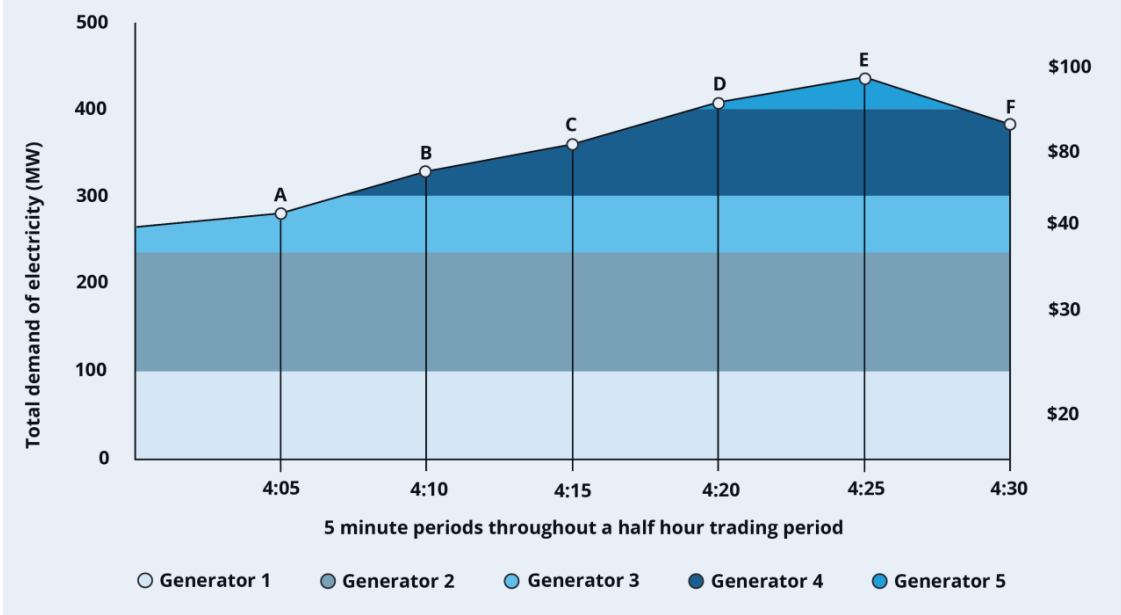
\includegraphics[width=0.7\textwidth]{Pictures/Chapter5/bidding.png}
    \caption{Scheduling generators in the NEM \parencite{AEMC_Bidding}}
    \label{fig:bidding_nem}
\end{figure}
\begin{center}
\begin{table}[]
\begin{tabular}{|l|l|l|l|l|}
\hline
\textbf{LOAD BID BAND}      & \textbf{Q1} & \textbf{Q2} & \textbf{Q3} & \textbf{Q4} \\ \hline
1                  & -988.6      & -988.6      & -988.6      & -985.3      \\ \hline
2                  & -500        & -500        & -500        & -500        \\ \hline
3                  & 0           & 0           & 0           & -50         \\ \hline
4                  & 30          & 30          & 30          & 25          \\ \hline
5                  & 60          & 60          & 60          & 50          \\ \hline
6                  & 90          & 90          & 90          & 90          \\ \hline
7                  & 150         & 120         & 150         & 120         \\ \hline
8                  & 300         & 150         & 300         & 150         \\ \hline
9                  & 1000        & 300         & 1000        & 300         \\ \hline
10                 & 5000        & 899         & 5000        & 899         \\ \hline
\textbf{GENERATOR BID BAND} & \textbf{Q1} & \textbf{Q2} & \textbf{Q3} & \textbf{Q4} \\ \hline
1                  & 90          & -984.8      & -970        & -977.1      \\ \hline
2                  & 150         & 0           & 0           & 0           \\ \hline
3                  & 200         & 90          & 90          & 60          \\ \hline
4                  & 250         & 120         & 120         & 90          \\ \hline
5                  & 300         & 200         & 200         & 175         \\ \hline
6                  & 450         & 300         & 300         & 250         \\ \hline
7                  & 600         & 450         & 450         & 400         \\ \hline
8                  & 1000        & 1000        & 1000        & 1000        \\ \hline
9                  & 5000        & 5000        & 5000        & 2000        \\ \hline
10                 & 13984.16    & 13500       & 13500       & 10027       \\ \hline
\end{tabular}
\end{table}
\end{center}
\begin{figure}
    \centering
    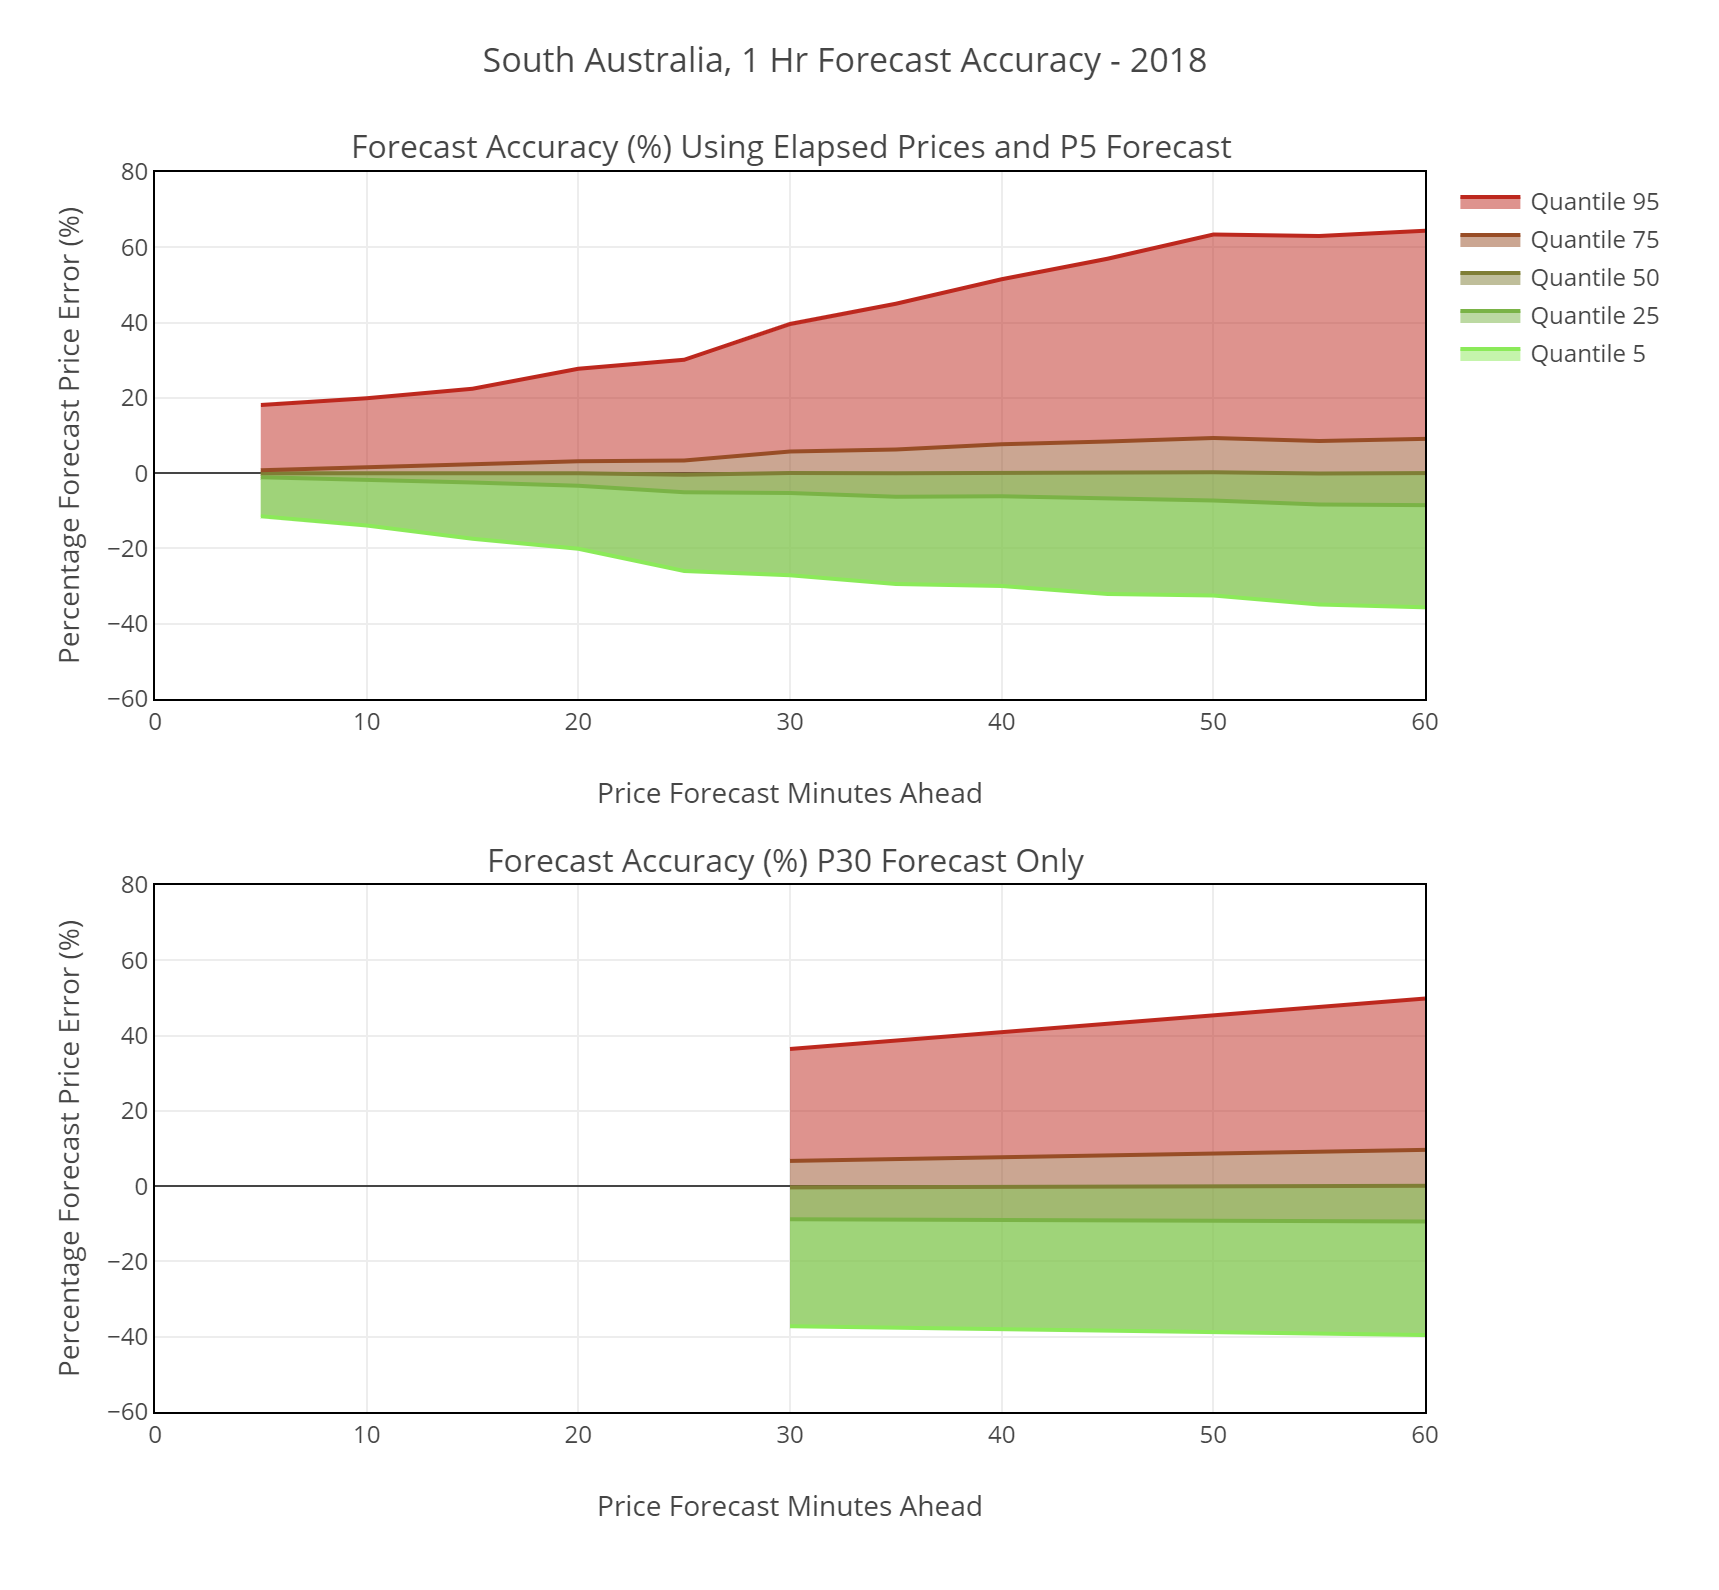
\includegraphics{Pictures/Chapter4/p30_p5_accuracy.png}
    \caption{Caption}
    \label{fig:my_label}
\end{figure}
\begin{figure}[H]
    \centering
    \makebox[\textwidth][c]{    \includegraphics[width=\textwidth]{"Pictures/Chapter5/Strategic_Bidding".pdf}}
    \caption{Caption}
    \label{fig:my_label}
\end{figure}


